%% This file is to be used as a template for your submission. 
%% Rename this file and replace the text with the text of 
%% your manuscript.
%%
%% The standard LaTeX document class "article" is recommended. 
%% Use options letterpaper and 12pt.
\documentclass[letterpaper,12pt]{article}\usepackage[]{graphicx}\usepackage[]{color}
%% maxwidth is the original width if it is less than linewidth
%% otherwise use linewidth (to make sure the graphics do not exceed the margin)
\makeatletter
\def\maxwidth{ %
  \ifdim\Gin@nat@width>\linewidth
    \linewidth
  \else
    \Gin@nat@width
  \fi
}
\makeatother

\definecolor{fgcolor}{rgb}{0.345, 0.345, 0.345}
\newcommand{\hlnum}[1]{\textcolor[rgb]{0.686,0.059,0.569}{#1}}%
\newcommand{\hlstr}[1]{\textcolor[rgb]{0.192,0.494,0.8}{#1}}%
\newcommand{\hlcom}[1]{\textcolor[rgb]{0.678,0.584,0.686}{\textit{#1}}}%
\newcommand{\hlopt}[1]{\textcolor[rgb]{0,0,0}{#1}}%
\newcommand{\hlstd}[1]{\textcolor[rgb]{0.345,0.345,0.345}{#1}}%
\newcommand{\hlkwa}[1]{\textcolor[rgb]{0.161,0.373,0.58}{\textbf{#1}}}%
\newcommand{\hlkwb}[1]{\textcolor[rgb]{0.69,0.353,0.396}{#1}}%
\newcommand{\hlkwc}[1]{\textcolor[rgb]{0.333,0.667,0.333}{#1}}%
\newcommand{\hlkwd}[1]{\textcolor[rgb]{0.737,0.353,0.396}{\textbf{#1}}}%
\let\hlipl\hlkwb

\usepackage{framed}
\makeatletter
\newenvironment{kframe}{%
 \def\at@end@of@kframe{}%
 \ifinner\ifhmode%
  \def\at@end@of@kframe{\end{minipage}}%
  \begin{minipage}{\columnwidth}%
 \fi\fi%
 \def\FrameCommand##1{\hskip\@totalleftmargin \hskip-\fboxsep
 \colorbox{shadecolor}{##1}\hskip-\fboxsep
     % There is no \\@totalrightmargin, so:
     \hskip-\linewidth \hskip-\@totalleftmargin \hskip\columnwidth}%
 \MakeFramed {\advance\hsize-\width
   \@totalleftmargin\z@ \linewidth\hsize
   \@setminipage}}%
 {\par\unskip\endMakeFramed%
 \at@end@of@kframe}
\makeatother

\definecolor{shadecolor}{rgb}{.97, .97, .97}
\definecolor{messagecolor}{rgb}{0, 0, 0}
\definecolor{warningcolor}{rgb}{1, 0, 1}
\definecolor{errorcolor}{rgb}{1, 0, 0}
\newenvironment{knitrout}{}{} % an empty environment to be redefined in TeX

\usepackage{alltt}

%% This is the recommended preamble for your document.
\usepackage{setspace}
\usepackage{url}
%% Load De Gruyter specific settings 
\usepackage{dgjournal}          
\usepackage{color,soul}
%% The mathptmx package is recommended for Times compatible math symbols.
%% Use mtpro2 or mathtime instead of mathptmx if you have the commercially
%% available MathTime fonts.
%% Other options are txfonts (free) or belleek (free) or TM-Math (commercial)
\usepackage{amssymb,amsmath}
\usepackage{multirow}
%% Use the graphics package to include figures
\usepackage{graphics}
%% Use natbib with these recommended options
\usepackage[authoryear,comma,longnamesfirst,sectionbib]{natbib} 
\usepackage{lscape}
\newcommand{\hlc}[2][yellow]{{\sethlcolor{#1}\hl{#2}}}
\setstretch{1}
\setlength{\bibsep}{10pt}
\usepackage{booktabs}

\usepackage{subfigure}% Support for small, `sub' figures and tables. Your choice of alternative may be preferred instead.
\usepackage{color,soul}
\usepackage{moreverb}
\usepackage{graphicx}
\usepackage[table]{xcolor}


%% Start your document body here
\IfFileExists{upquote.sty}{\usepackage{upquote}}{}
\begin{document}

\begin{center} Are hot streaks in baseball pitchers real?  Mhmm.
\end{center}


\begin{abstract} 
In the past, ``Hot streaks" in sports have been notoriously difficult to demonstrate despite the fact that many players across many different sports are convinced that they exist.  Here we consider looking for streakiness in starting pitchers in major league baseball by examining a statistic that the pitcher has almost complete control over: fastball velocity.  We fit a mixed hidden Markov model (HMM) in a Bayesian framework using the sequences of fastball velocities generated by starting pitchers. This model allows for parameters of the emission distributions and the transition matrices to vary by player while simultaneously allowing for pooling information across players.  We begin by fitting a two state model and find evidence that there is approximately a 2-3 MPH difference between the states, on average.  Further, we study the predictive effects of our model and find that ``hot" pitchers outperform ``cold" pitchers in future starts in such statistical categories such as strikeouts and ERA.  We also find evidence that when a pitcher is ``hot" based on their fastball that other pitches are also improved (e.g. curveball). 

  \end{abstract}

\doublespacing





\title{Hot streaks are real, bitches!}

%\author{Gregory J. Matthews,$^{\rm a}$$^{\ast}$\thanks{$^\ast$Corresponding author. Email: gmatthews1@luc.edu
%\vspace{6pt}} P\'{e}tala Gard\^{e}nia da Silva Estrela Tuy,$^{\rm a}$ and Robert Arthur$^{\rm b}$\\
%\vspace{6pt}  $^{a}${\em{Department of Mathematics and Statistics, Loyola University Chicago, 1032 W. Sheridan Road, Chicago, IL USA}};\\
%\vspace{6pt}  $^{b}${\em{FiveThirtyEight, 147 Columbus Ave., 4th Floor, New York, NY 10023}};
%\\\received{Received: XX Month 2016; accepted XX Month 2016} }

%\maketitle


%\begin{keywords}Statistical Disclosure; Multiple Imputation; Latent Class Analysis; Baseball 
%\end{keywords}

%\begin{classcode}\textit{Classification codes}: 	62P99; 62-07 \end{classcode}

%\end{abstract}
\section{Introduction}
\subsection{The ``Hot Hand"}
%Outline
%Intro and lit review on hot hand stuff.  
%Methods: Describe Mixture models, Hidden markov models, then mixed HMM in general
%Data: Describe the data
%Describe OUR specific model
%Model fit results: posterior predictive checks.  convergence checks.  
%results: parameter estimates, present some pitchers.  
% COnclsuions and future work


There is a rich collection of literature studying the concept of ``streakiness" or ``hot hand" effect in sports and many classic research papers looking into the topic have concluded that this effect does not actually exist.  The seminal work in this area is \cite{Gilovich1985}, which studied the ``hot hand" in basketball using shot data from the Philadelphia 76ers and free throws from the Boston Celtics, both of the National Basketball Association (NBA), along with free throw data collected under experimental conditions from Cornell's men's and women's varsity basketball teams.  Based on their analysis they conclude that the hot hand in shooting does not exist, even referring to it as a ``cognitive illusion" (\cite{Gilovich1985}, Page 313).  Additional work in this line of research supporting the idea that the hot hand is merely an illusion can be found in \cite{HuizingaWeil2009,TverskyGilovich1989,KoehlerConley2003}.  More recently, however, the orthodoxy that the ``hot hand" is not real is beginning to challenged as access to newer and larger data becomes available to researchers.  For example, \cite{Arkes2010} uses data from every free throw occurring in the 2005-06 season of the National Basketball Association (NBA),  and they find a 2-3\% increase in the probability of making the second free throw given that the first free three is made. \cite{Arkes2013}, continuing to focus on free throws, performs a simulation study to demonstrate that the primary methods (e.g. runs test and tests for stationarity) for detecting the hot hand in past studies (such as \cite{HuizingaWeil2009,Gilovich1985,TverskyGilovich1989,KoehlerConley2003}) may not be adequate for detecting the hot hand.  For instance, \cite{Arkes2013} estimates that if the frequency of the hot hand is 20\%, the true hot hand effect was 10 percentage points and the overall probability of making a free throw is 75\% (i.e. probability of making a shot when hot is 83\%; probability of making a shot when cold is 73\%), there is only a 5.2\% chance that the hot hand will be detected with a sample size of 2,160.  When the sample size is increased to 28,800, there is still only a 33.0\% chance of detecting the hot hand under these parameter conditions.  

Moving beyond only free throws in basketball, \cite{BocskocskyEtAl2014} looked at approximately 83,000 field goal attempts from the 2012-2013 NBA season.  After conditioning on the difficulty of the shot, they estimate the effect of the hot hand to be between 1.2 and 2.4 percentage points.  

\cite{BarEliEtAl2006}: This paper is a literature review of the hot hand across all sports.  
ALl quotes from BarEliEtAl2006
Baseball batting: 
Siwoff et al. (1988) Batting averages before and after a hot streak.  
Gould (1989) Dimaggio hit streak. 
Albright (1993) 1. Some players exhibited significant streakiness
during a given season, but this would be
expected under a model of randomness.
2. Not a single one of these players exhibited
significantly streaky behavior over the entire 4-
year period.

Stern (1995): Evidence of streaks was found while players were analyzed as a group rather than individually.
This is in the JSM proceedings.  Where the hell do I get that from 1995? 

Albert and Bennett (2001): Zeile exhibited both ``hot" and ``cold"
performances, but the peaks and valleys observed
in batting average would be due just to chance.

Baseball pitching: 
Frohlich (1994) : No hitters and their distribution


Baseball teams streaks: 
Vergin(2000) Wins and losses were shown to be independent of
the results of previous games and winning and
losing streaks were no longer than would be
expected by chance.

Golf:
Clark 2003a and 2003b: differences attributed to difficulty of course.  

Basketball: 
Koehler and Conley (2003): 23 shooters in four annual NBA Long Distance
Shootout contests, 1994–1997 (a total of 56 sets of 25 shots). Greg comment: Very small sample size.

Forthofer (1991): Of the 123 players examined, there were 17 that
could be labeled streak shooters (i.e., 5\% or more
of the total number of games were inconsistent
with the player’s season field goal percentage),
with an emphasis on three players.
____________

A lot of the previous work that has been done was looking at streak in the success/failure of an event (e.g. putts, baskets, hits).  Out approach is fundamentally different.  We are looking at streaks in a continuous outcome.  

Basketball.  
Gilovich 1989

Debate the findings:  
Tversky and Gilovich 1989
Larkey Smith and Kadane 1989
Hooke 1989

% \cite{Arkes2010} Hot hand in basketball in free throws.  Using ALL free throws across a season and controlling to other factors.  There is a 2-3\% increase in the probability of hitting the second free throw given that the first free throw is hit.  

% \cite{Arkes2013}: From this paper ``Indeed, several studies have used simulation models to demonstrate that when a hot hand does exist, the common tests used in prior studies, particularly the
% runs test and the test for stationarity?which were used by Gilovich et al. (1985),
% Tversky and Gilovich (1989), and Koehler and Conley (2003)?would not detect
% statistical significance most of the time (Dorsey-Palmateer & Smith, 2004; Frame
% et al., 2003;Miyoshi, 2000; andWardrop, 1999)."

% Bocskocsky et al (2014): Using a data set of 83000 shots from the NBA 2012-2013 season, they show that conditional on shot difficultty that ``palyers for are outperforming continute to do so."  They estimate the ``hot hand effect to be in the range of 1.2 to 2.4 percentage points in increased likelihood of making a shot."

Post error and hot hand.  http://journal.sjdm.org/15/15914a/jdm15914a.html

Another paper that does not find hot hand.  Avugos, Köppen, Czienskowski, Raab & Bar-Eli, 2013

\cite{RabinVayanos2010} Economics paper on hot streaks in markets.  

\cite{BarEliEtAl2006} Find little empirical evidence to support the hot hand 
Bar-Eli, Michael, et al. “Twenty Years of ‘Hot hand’ Research: Review and Critique.” Psychology of Sport and
Exercise 7, no. 6 (2006): 525-553.


Rao, Justin M. “Experts’ Perceptions of Autocorrelation: The Hot Hand Fallacy Among Professional Basketball
Players.” 2009

\cite{Albright1993} Hittin streaks.  Some players exhibit streaky behavior.  But most don't. and none over a 4 year period.  Looked at MLB "regular" players from 1987 -1990.  Uses a "runs test" and logistic regression.  Taken as a whole however, the streakiness does not differ significantly from randomness.  


``The 1988 version of {\em The Elias Baseball Analyst} reports its own study of streakiness for 1984-1987"

Gould 1989 is more philosophical that quantitiative.  



Green and Zweibel 2016: Find effects of the hot hand.  

Arkes 2013: Need to get thi spaper.    Simulation study shows that the way studies are done that even detecting a small effect actually is evidence of a muhc larger effect.  

Bowler's Hot Hands: 
%\cite{Stone2012}:



Arkes 2013 identifies three possibl issues: 1) Power/sample size, 2)It's a measurement error problem.  The shots are recorded as 0 or 1, but there are underlying probabdilities 3) Frequency of hot hand events it low.  

We propose to use a hidden markov model to look for players in different states.  These states good be ``hot" and ``cold" or something like that (i.e. ``locked in" or ``not locked in").  This could also be ``injured" versus ``not injured. 

So we have longitudinal data from multiple pitchers.  And we are hypothesizing that this data is generated from one of two hidden states.  We could view this data as arising from a mixture model however, that would ignore the time dependence of the data.  HMM allow for modeling data arising from a mixture distribution along with serial dependence in the data.  A single HMM is therefore well suited for modeling each time series of each pitcher performance individually.  However, our goal is to pool all these time series together to "borrow information" across pitchers to estimate league wide parameters for hot and cold.  

\subsection{Mixture Models, Hidden Markov Models, and Mixed Hidden Markov Models}
Mixture models (CITE) fit data that are assumed to be generated from multiple processes, which is useful in the current application, as it is hypothesized that the data (i.e. adjusted fastball velocities) are being generated from two distinct states (i.e. ``hot" and ``cold").  However, mixture models assume independence between observations and do not account for serially correlated data.  

\begin{figure}[ht]
		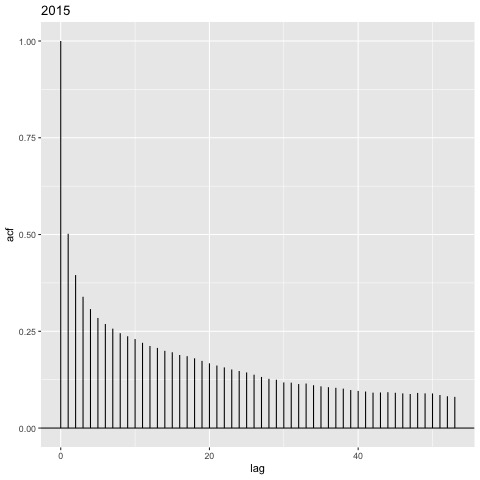
\includegraphics[width=0.3\linewidth]{../fig/acf2015.jpg}
		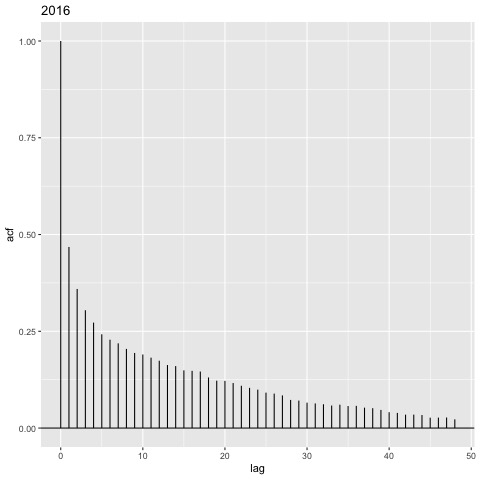
\includegraphics[width=0.3\linewidth]{../fig/acf2016.jpg}
	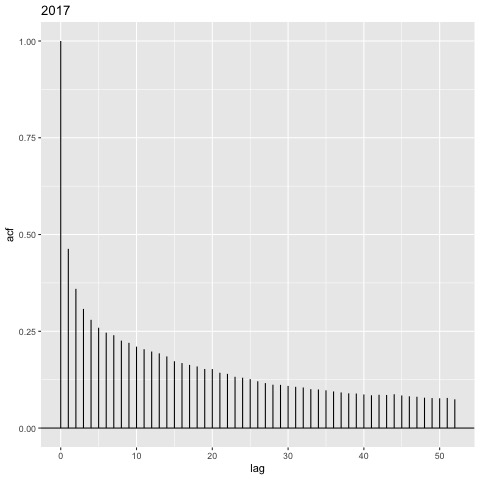
\includegraphics[width=0.3\linewidth]{../fig/acf2017.jpg}

	  \caption{Autocorrelation plot for 2015, 2016, and 2017 for adjusted fastball velocities (i.e. residuals from the linear model.}
  \label{acf}
\end{figure}

Hidden Markov Models (HMM) blah blah



\cite{Humphreys1998} and \cite{Seltman2002} both present work that deals with multiple sequences at once.  Later, in \cite{Altman2007} the methods described in the aforementioned articles are formalized and the term mixed hidden Markov models (MHMM) is applied to describe models of this type.   Further work applying this method can be found in \cite{ShirleyEtAl2010}, which presents an application of the MHMM framework in the context of a clinical trial.  An overview of MHMM can be found in \cite{Maruotti2011}.  

\cite{Altman2007}
\cite{MeedenAndVardeman1997}


\section{Data}
For pitchers we are looking at fastball velocities.  We are using data from the DATA BASE NAME.  We looked at  starting pitchers from the major league baseball (MLB) during the regular season and we look at the 2015, and 2016, and 2017 seasons separately.  In this analysis we included all pitches where the pitch type is listed as a fastball or pitch type is listed as a cutter and is classified as hard. 

This data set contains 308 unique pitchers who threw a total of 253,462 pitches.  After removing observation with missing values, 253,244 observations remain.  We then filter to include only pitchers who threw more than 800 pitches during the 2016 season.  This leaves us with 136 pitchers and 199,975 pitches.  


%\begin{figure}[ht]
%	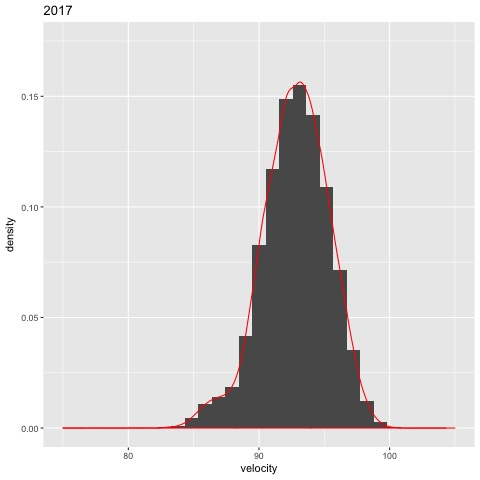
\includegraphics[width=0.5\linewidth]{velHist2017.jpg}
%	  \caption{Distribution of pitch velocities}
%  \label{fig:hist}
%\end{figure}

\begin{figure}[ht]
		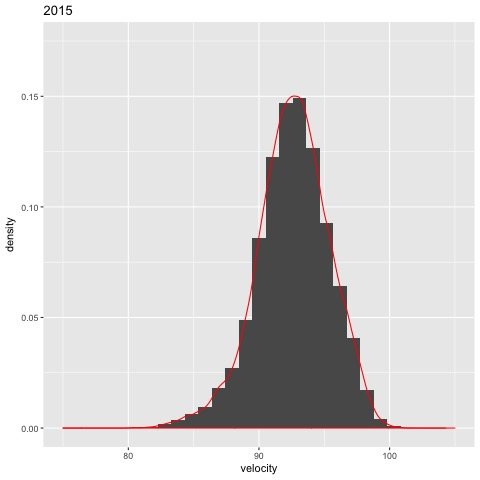
\includegraphics[width=0.3\linewidth]{velHist2015.jpg}
		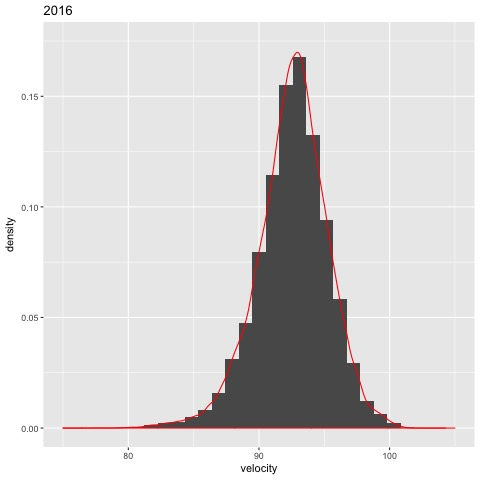
\includegraphics[width=0.3\linewidth]{velHist2016.jpg}
	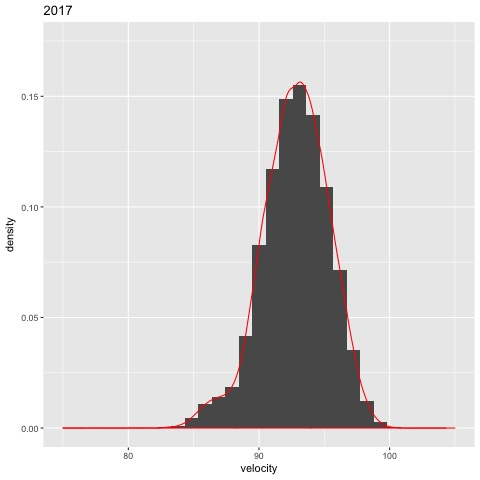
\includegraphics[width=0.3\linewidth]{velHist2017.jpg}

	  \caption{Histogram of velocities for 2015, 2016, and 2017}
  \label{acf}
\end{figure}

%begin{figure}[ht]
%	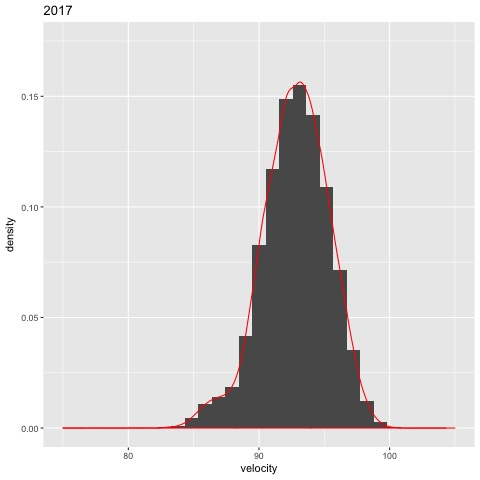
\includegraphics[width=0.5\linewidth]{velHist2017.jpg}
%	  \caption{Distribution of pitch velocities}
%  \label{fig:hist}
%\end{figure}

\begin{figure}[ht]
		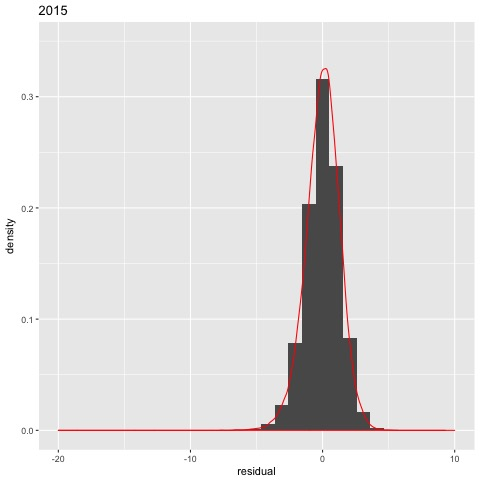
\includegraphics[width=0.3\linewidth]{residHist2015.jpg}
		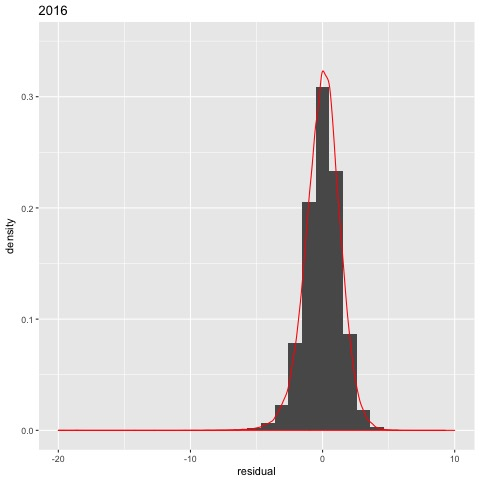
\includegraphics[width=0.3\linewidth]{residHist2016.jpg}
	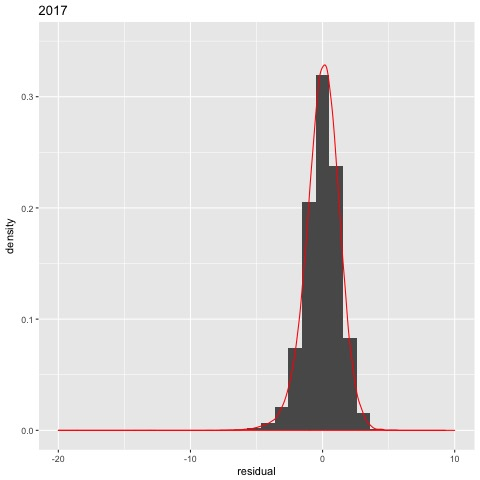
\includegraphics[width=0.3\linewidth]{residHist2017.jpg}
	  \caption{Histogram of residuals for 2015, 2016, and 2017}
  \label{acf}
\end{figure}

2015 data: 263186 observations
After cleaning:  212190.  

2016 Data: 253462
After cleaning 199975


2017 Data: 244057
After cleaning: 190529




\section{Model}
\subsection{Controlling external effect}
%This can either be done for batters or pitchers.  For batters we use batted ball velocity as the emissions from the states and for pitchers we use fastball velocity.  In both of these situations, we first control for external variables that may have an effect on these two velocities.  For instance, for pitchers we control for how many pitches they have thrown (among other variables). We then use the adjusted velocities after controling for these external factors is what we use as emissions in our hidden markov model.
The overall goal of this model is to measure for a pitcher performs relative to their own average performance.  That is, this model seeks to find strings of pitches where a pitcher is better than their average (i.e. ``hot") or worse than their average (i.e. ``cold").  Therefore, a model to control for effects that are external to the pitcher is fit first prior to the HMM.  This model is a linear mixed effects model with fixed effects for pitch type, pitch count, an indicator for baserunners, elevation, and temperature.  (Note: The three pitch types include fastballs, ``hard" cutters, and sinkers, which are all meant to be thrown as hard as possible, as opposed to, for instance, a change up or a curve ball).  Interactions between pitch type and pitch count, pitch type and baserunners, and elevation and temperature were also included in this model.  Finally, a random in intercept was included for all pitchers to establish a baseline velocity for each.   This model can be expressed as: 

$$
v_{tj} = \delta_0 + {\bf \delta} X_{tj} + d_{j} + \epsilon_{tj}
$$

$$
\epsilon_{tj} \sim N(0,\sigma_{epsilon})
$$

$$
\d_{j} \sim N(0,\sigma_{d})
$$

where $\delta_0$ is the fixed intercept of the model, ${\bf \delta}$ is a vector of fixed effects,  $d_{j}$ is the random effect for the $j$-th pitcher, $v_{tj}, $X_{tj}$, $\epsilon_{tj}$ are the velocity, a vector of covariates, and the residual, respectively, of the $t$-th pitch for the $j$-th pitcher and $j=1\cdots J$ and $t=1\cdots T_{j}$.  

$\epsilon_{tj}$ can be interpreted as the velocity above or below expectation for pitcher $j$ (i.e. when $\epsilon_{tj}=0$ this indicates that the velocity of pitch $t$ for pitcher $j$ is exactly average given that pitcher and set of external factors).  This string of residuals will be searched to look for stretches that are more positive that usual (i.e. a ``hot" streak) or more negative than usual (i.e a ``cold" streak).  
This search will be accomplished by viewing these residuals ($epsilon_{tj}$) as the emissions from a  hidden Markov model. 

\subsection{MHMM}
This project is interested in looking for ``hot" and `cold" states of pitchers, therefore, a two-state hidden Markov model is chosen to look for evidence of these two proposed states.  Now, a separate two state hidden Markov model could be fit for each pitcher $j$ yielding $J$ different models, one for each pitcher.  Rather, one model will be fit using all the data at once with a random effect to account for differences between pitchers. 



This type of model, termed a mixed hidden Markov model (MHMM), is described in \cite{Altman2007}. 

  
%Assumptions from ALtman: 
%I make the following additional assumptions:
%1. Zit takes on values from a finite set, {1, 2, . . . ,K}, where K is known.
%2. Given the random effects, {Zit}ni t=1 are Markov chains. These processes may or may not be stationary.
%3. Conditional on the random effects, the ith process,{Yit}ni t=1, is a HMM, and




$$
\epsilon_{tj} \sim Normal(\mu_{tj},\sigma^2) 
$$
where $\tau^2=\frac{1}{\sigma^2}$
$$
\mu_{tj} = (\beta_1 + b_{j1})\mathcal{I}(S_{tj}=1) + (\beta_2 + b_{j2})\mathcal{I}(S_{tj}=2) 
$$
$$
S_{tj} \sim Bern(p_{tj}) + 1
$$
$$
logit(p_{tj}) =(\gamma_1 + g_{j1})\mathcal{I}(S_{(t-1)j}=1) + (\gamma_2 + g_{j2})\mathcal{I}(S_{(t-1)j}=2)
$$
$$
\beta_{1} \sim Uniform(-20,20)
$$

$$
\beta_{2} \sim Uniform(\beta_1,20) 
$$

$$
b_{j1} \sim Uniform(-20,20)
$$
$$
b_{j2} \sim Uniform(b_{j1}+\beta_1-\beta_2,20) 
$$
$$
g_{j1} \sim Uniform(-7,7);g_{j2} \sim Uniform(-7,7)
$$
$$
\gamma_1 \sim Uniform(-7,7);
\gamma_2 \sim Uniform(-7,7)
$$
$$
\tau^2 \sim \Gamma(0.001,0.001);
$$





$S_{0j}$ is the initial state for the $j$-th player and $S_{tj}$ is the state at time $t$ for player $j$.  $\beta_1$  and $\beta_2$ are the means of the emission distributions for an average pitcher in state $1$ and $2$, respectively, and $\beta_2$ is forced to be larger than $\beta_1$.  $b_{j1}$ and $b_{j2}$ are the player specific effects for the means of the emissions in states $1$ and $2$, respectively.  Additionally, the model requires that $\beta_2 + b_{j2} \ge \beta_1 + b_{j1}$.  



The transition matrix is defined by the $\gamma$'s and the $g$'s.  
The transition probabilities are: 
 $$\nu_{1,2,j} = P(S_{tj}=2 | S_{(t-1)j}=1) = expit(\gamma_1 + g_{j1})$$
  $$\nu_{1,1,j} =  P(S_{tj}=1 | S_{(t-1)j}=1) = 1-P(S_{tj}=2 | S_{(t-1)j}=1)$$

 $$\nu_{2,2,j} =  P(S_{tj}=2 | S_{(t-1)j}=2) = expit(\gamma_2 + g_{j2})$$
  $$\nu_{2,1,j} = P(S_{tj}=1 | S_{(t-1)j}=2) = 1-P(S_{tj}=2 | S_{(t-1)j}=2)s
  $$
  
  The transition matrix for the $j$-th individual is 
  $$
  \Gamma_j = \left(\begin{array}{cc}
\nu_{1,1,j} & \nu_{1,2,j} \\
\nu_{2,1,j} & \nu_{2,2,j}\\
\end{array}\right)
  $$



\section{Results}
10 chains of 10000 draws each were run for all of the parameters.  The first 9000 draws were then thrown out of each chain.  

In 2015, 6 of the chains needs to be thrown out because they failed to converge for beta.  

\begin{figure}[ht]
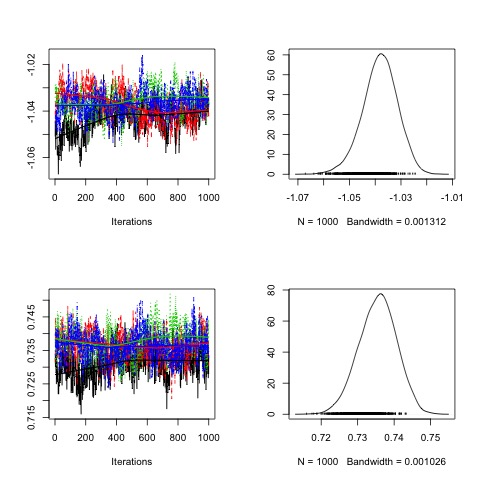
\includegraphics[width=0.3\linewidth]{betaPosterior2015.jpg}
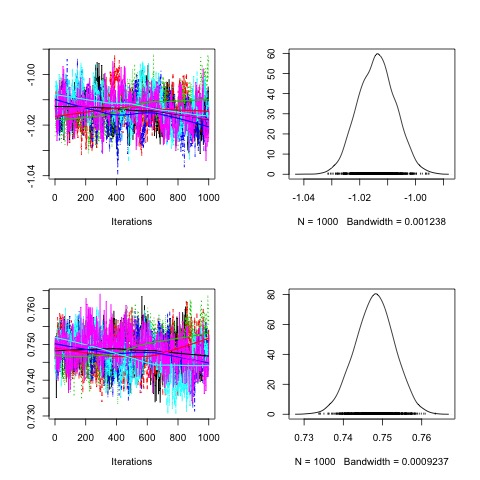
\includegraphics[width=0.3\linewidth]{betaPosterior2016.jpg}
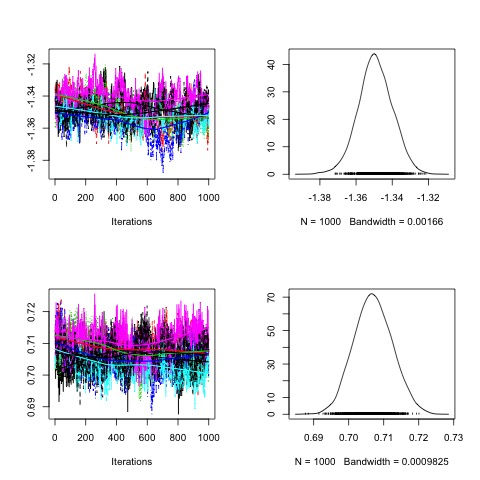
\includegraphics[width=0.3\linewidth]{betaPosterior2017.jpg}
	  \caption{Trace plots of the posterior distribution of $\beta$}
  \label{betaPosterior}
\end{figure}


\begin{figure}[ht]
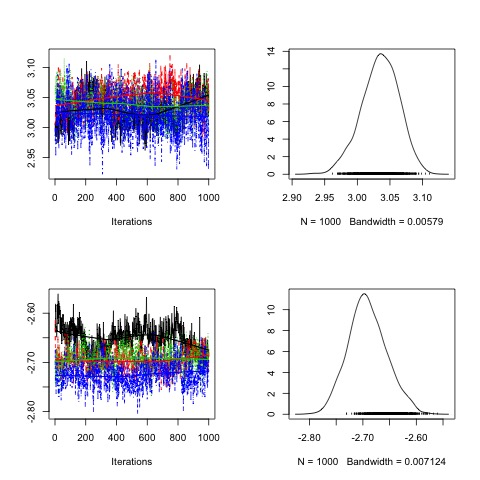
\includegraphics[width=0.3\linewidth]{gammaPosterior2015.jpg}
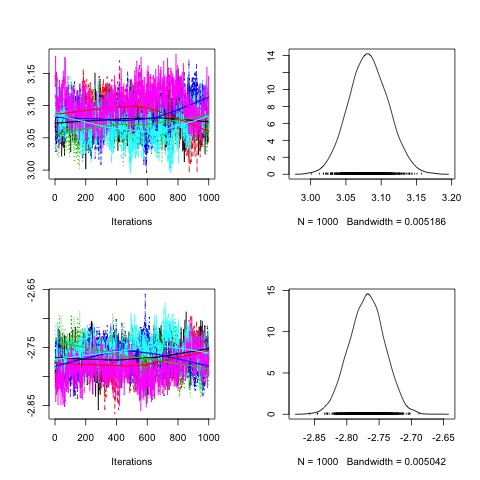
\includegraphics[width=0.3\linewidth]{gammaPosterior2016.jpg}
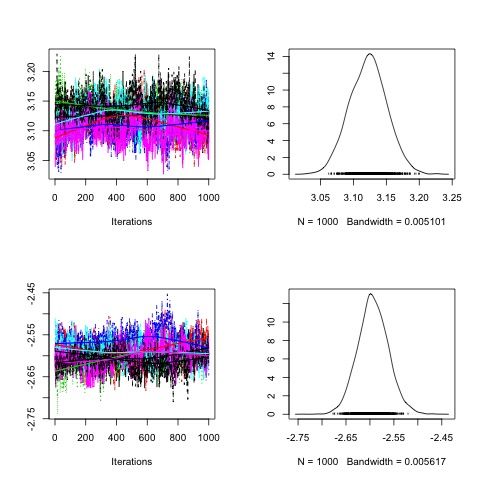
\includegraphics[width=0.3\linewidth]{gammaPosterior2017.jpg}
	  \caption{Trace plots of the posterior distribution of $\gamma$}
  \label{betaPosterior}
\end{figure}






\subsection{Model Diagnostics}
Posterior predictive checks and Gelman convergence plots and trace plots.  


In all three years, first 5000 draws we run as a burn-in period and then another 10000 draws were run.  Based on inspection of the trace plots 5000 is not enough to reach convergence and and additional 9000 of the 10000 draws were removed.  Finally, each chain was checked for convergence visually and chains that still did not appear to converge were removed. 

\subsubsection{2015}
First 5000 draws we run as a burn-in period and then another 10000 draws were run.  Based on inspection of the trace plots 5000 is not enough to reach convergence and and additional 9000 of the 10000 draws were removed.  Finally, each chain was checked for convergence visually and chains that  still did not appear to converge were removed.  In 2015 four chains were left.  The gelman plot for 2015 can be seen and the Gelman diagnostic for the last 1000 draws of 4 chains is beta1 = 1.36 (upper CI 1.86), beta2 = 1.33 (upper CI 1.79).  Gamma1 = 1.22 (1.58) and gamma2 = 1.86 (2.88).  Tau = 1.03 (1.1).  

\subsubsection{2016}
 In 2016 four chains were removed.  The gelman plot for 2016 can be seen and the Gelman diagnostic for the last 1000 draws of 6 chains is beta1 = 1.07 (upper CI 1.16), beta2 = 1.13 (upper CI 1.29).  Gamma1 = 1.19 (1.42) and gamma2 = 1.14 (1.32).  Tau = 1.04 (1.09).  


\subsubsection{2017}
 In 2017 three chains were removed.  The gelman plot for 2017 can be seen and the Gelman diagnostic for the last 1000 draws of 7 chains is beta1 = 1.22 (1.48), beta2 = 1.17 (1.36).  Gamma1 = 1.21 (1.44) and gamma2 = 1.25 (1.51).  Tau = 1.03 (1.06).  


This paper suggests that the Gelman diagnostic should be below 1.2 for all parameters to demonstrate convrgence.  We have some problems with that in 2015.  
Brooks, S. P., and A. Gelman. 1997. General Methods for Monitoring Convergence of Iterative Simulations. Journal of Computational and Graphical Statistics 7: 434–455.

Gelman, A., and D. B. Rubin. 1992. Inference from Iterative Simulation Using Multiple Sequences. Statistical Science 7: 457–511.





\subsection{Parameter Estimates}

{\tiny
%Posterior Means  with 95% credible interval
\begin{center}
\begin{tabular}{cccccc}
Year & $\beta_1$  & $\beta_2 & $\gamma_1$ & $\gamma_2$ & $\tau$\\ 
2015 & -1.038 (-1.052, -1.026) & 0.736 (0.725, 0.745) & 3.035 (2.975, 3.088) & -2.691 (-2.758, -2.616) & 0.947 (0.940, 0.954) \\ 
2016 & -1.014 (-1.0266, -1.0009) & 0.748 (0.7381, 0.7575) &3.082 (3.029, 3.138)& -2.769 (-2.822, -2.717) & 0.9109 (0.9039, 0.9179)\\ 
2017 & -1.349 (-1.3681, -1.3307) & 0.707 (0.6967, 0.7178)& 3.122 (3.067, 3.178) & -2.593 (-2.655, -2.529) (& 0.8938 (0.8869, 0.9010)\\
\end{tabular}
\end{center}
}

\begin{figure}
\begin{center}
\begin{tabular}{ |c| c| c| }
\hline
 & To Hot  & To Cold \\ 
 \hline
From Hot & 0.95413544 & 0.04586456 \\  
\hline
From Cold & 0.06349286 & 0.93650714    \\
\hline
\end{tabular}
\end{center}
\caption{2015 Transition Matrix}
\end{figure}

\begin{figure}
\begin{center}
\begin{tabular}{ |c| c| c| }
\hline
 & To Hot  & To Cold \\ 
 \hline
From Hot &0.95615461 &  0.04384539  \\  
\hline
From Cold &0.05902627 &  0.94097373   \\
\hline
\end{tabular}
\end{center}
\caption{2016 Transition Matrix}
\end{figure}

\begin{figure}
\begin{center}
\begin{tabular}{ |c| c| c| }
\hline
 & To Hot  & To Cold \\ 
 \hline
From Hot &0.95780989 & 0.04219011  \\  
\hline
From Cold &0.06956167 & 0.93043833   \\
\hline
\end{tabular}
\end{center}
\caption{2017 Transition Matrix}
\end{figure}

\begin{figure}[ht]
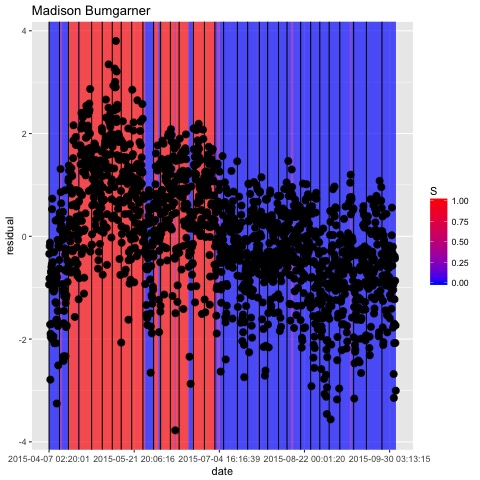
\includegraphics[width=\linewidth, height=2in]{Bumgarner2015.jpg}
	  \caption{Trace plots of the posterior distribution of $\beta$}
  \label{betaPosterior}
\end{figure}

%There is a file called AnalysingDataAfterDrawsOnServer2.R that generates these files.  
%Plot of Kershaw over the 2015 season
\begin{knitrout}
\definecolor{shadecolor}{rgb}{0.969, 0.969, 0.969}\color{fgcolor}
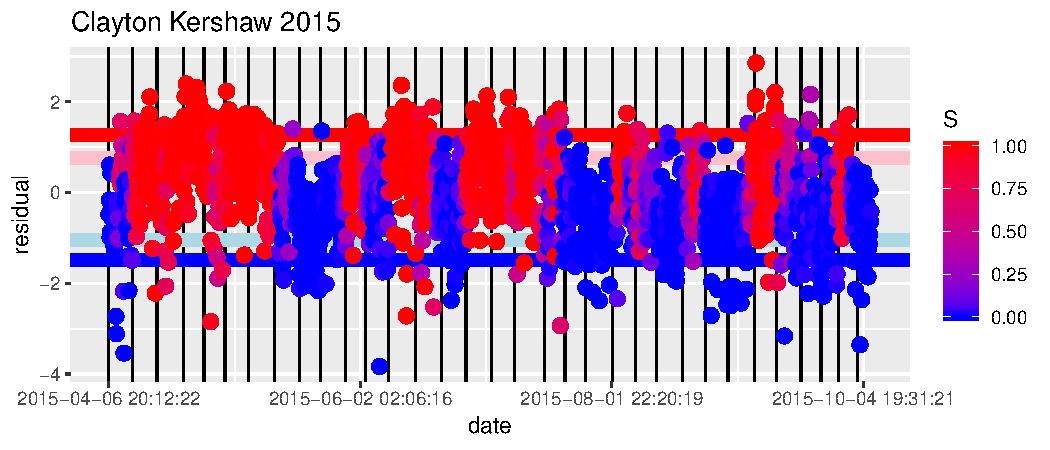
\includegraphics[width=\maxwidth]{figure/unnamed-chunk-1-1} 

\end{knitrout}


%Plot of Kershaw over the 2016 season
\begin{knitrout}
\definecolor{shadecolor}{rgb}{0.969, 0.969, 0.969}\color{fgcolor}
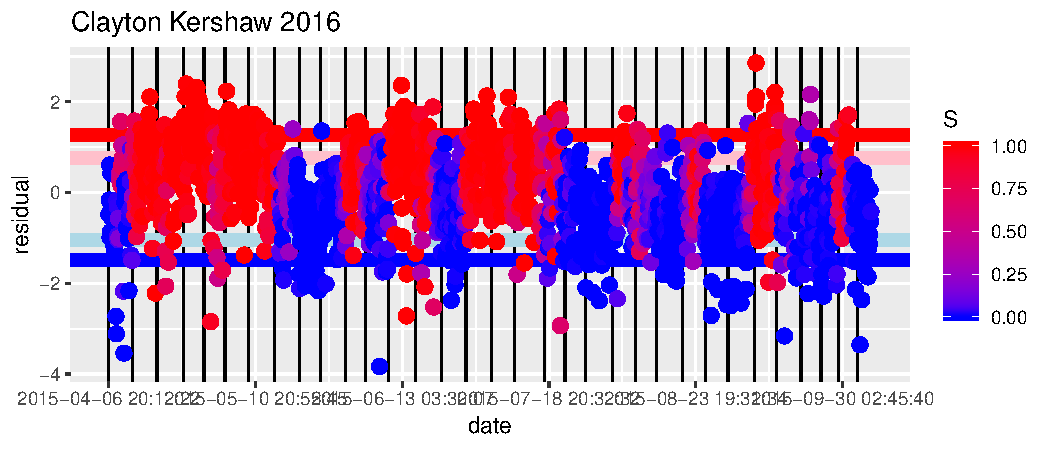
\includegraphics[width=\maxwidth]{figure/unnamed-chunk-2-1} 

\end{knitrout}


%Plot of Kershaw over the 2017 season
\begin{knitrout}
\definecolor{shadecolor}{rgb}{0.969, 0.969, 0.969}\color{fgcolor}
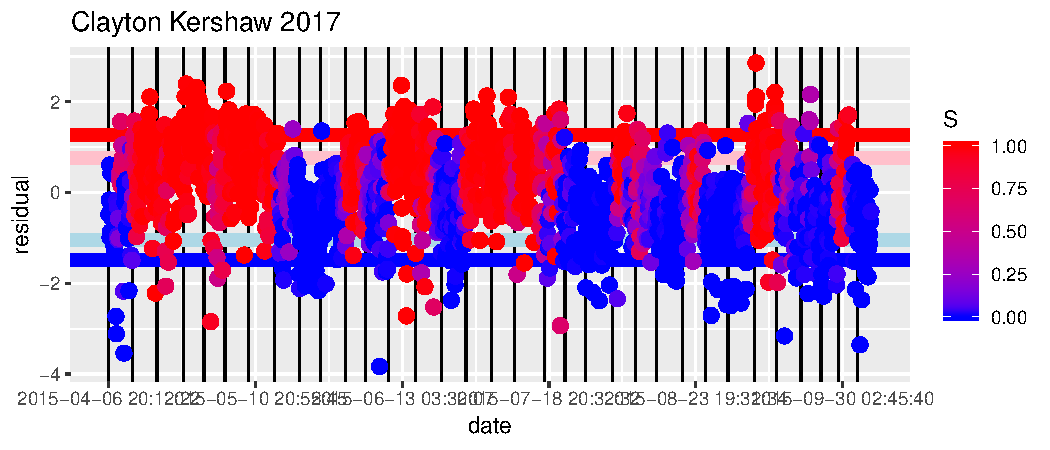
\includegraphics[width=\maxwidth]{figure/unnamed-chunk-3-1} 

\end{knitrout}

\subsection{Prediction}
Once the model has been fit, posterior means of each of the parameters can be used as a point estimate.  The betas, gammas, and tau are parameters that apply to all players and b and g are parameters that are player specific.  Using all of these point estimates, a Hidden Markov model can be constructed based on the posterior estimates.  

Prediction with Viterbi2.  


\section{Conclusions and Future Work}
The lag doesn't seem long enough to really fit the data well.  A more complex model is probably needed.  We view this paper as a starting point.  Buchholz is an interesting example in 2016.  


\section*{Appendix}
2015 Model Fixed Effects
% latex table generated in R 3.4.0 by xtable 1.8-2 package
% Wed Dec 13 11:23:10 2017
\begin{table}[ht]
\centering
\begin{tabular}{rrrr}
  \hline
 & Estimate & Std. Error & t value \\ 
  \hline
(Intercept) & 92.65 & 0.2018 &   459 \\ 
  pi\_pitch\_typeFC & -2.429 & 0.03261 & -74.47 \\ 
  pi\_pitch\_typeSI & -0.3927 & 0.01311 & -29.95 \\ 
  pitch\_count & -0.002428 & 0.0001333 & -18.22 \\ 
  baserunnersTRUE & 0.2647 & 0.00817 & 32.39 \\ 
  elevation & -7.142e-05 & 2.121e-05 & -3.368 \\ 
  gtemp & 0.002234 & 0.0003488 & 6.404 \\ 
  pi\_pitch\_typeFC:pitch\_count & -0.003438 & 0.0004977 & -6.907 \\ 
  pi\_pitch\_typeSI:pitch\_count & -0.002411 & 0.0002105 & -11.45 \\ 
  pi\_pitch\_typeFC:baserunnersTRUE & -0.1494 & 0.0286 & -5.223 \\ 
  pi\_pitch\_typeSI:baserunnersTRUE & -0.002739 & 0.01264 & -0.2167 \\ 
  elevation:gtemp & 8.037e-07 & 2.885e-07 & 2.786 \\ 
   \hline
\end{tabular}
\end{table}


2016 Model Fixed Effects
% latex table generated in R 3.4.0 by xtable 1.8-2 package
% Wed Dec 13 11:21:30 2017
\begin{table}[ht]
\centering
\begin{tabular}{rrrr}
  \hline
 & Estimate & Std. Error & t value \\ 
  \hline
(Intercept) & 92.43 & 0.1932 & 478.4 \\ 
  pi\_pitch\_typeFC & -2.935 & 0.04205 & -69.8 \\ 
  pi\_pitch\_typeSI & -0.3944 & 0.01367 & -28.86 \\ 
  pitch\_count & -0.001894 & 0.000136 & -13.93 \\ 
  baserunnersTRUE & 0.2234 & 0.008291 & 26.95 \\ 
  elevation & 1.33e-05 & 2.277e-05 & 0.5843 \\ 
  gtemp & 0.006481 & 0.0003472 & 18.67 \\ 
  pi\_pitch\_typeFC:pitch\_count & -0.00587 & 0.0006511 & -9.016 \\ 
  pi\_pitch\_typeSI:pitch\_count & -0.002994 & 0.0002215 & -13.52 \\ 
  pi\_pitch\_typeFC:baserunnersTRUE & 0.01535 & 0.03731 & 0.4114 \\ 
  pi\_pitch\_typeSI:baserunnersTRUE & 0.0503 & 0.0132 &  3.81 \\ 
  elevation:gtemp & -2.404e-07 & 2.981e-07 & -0.8064 \\ 
   \hline
\end{tabular}
\end{table}

2017 Model Fixed Effects
% latex table generated in R 3.4.0 by xtable 1.8-2 package
% Wed Dec 13 11:28:36 2017
\begin{table}[ht]
\centering
\begin{tabular}{rrrr}
  \hline
 & Estimate & Std. Error & t value \\ 
  \hline
(Intercept) & 93.04 & 0.1779 & 523.1 \\ 
  pi\_pitch\_typeFC & -2.96 & 0.04273 & -69.26 \\ 
  pi\_pitch\_typeSI & -0.6632 & 0.01424 & -46.56 \\ 
  pitch\_count & -0.00335 & 0.0001399 & -23.94 \\ 
  baserunnersTRUE & 0.1913 & 0.008494 & 22.52 \\ 
  elevation & 4.565e-05 & 2.008e-05 & 2.273 \\ 
  gtemp & 0.001481 & 0.0003866 & 3.831 \\ 
  pi\_pitch\_typeFC:pitch\_count & -0.004052 & 0.0006807 & -5.953 \\ 
  pi\_pitch\_typeSI:pitch\_count & -0.001141 & 0.0002302 & -4.959 \\ 
  pi\_pitch\_typeFC:baserunnersTRUE & 0.06236 & 0.039 & 1.599 \\ 
  pi\_pitch\_typeSI:baserunnersTRUE & 0.1241 & 0.01366 & 9.079 \\ 
  elevation:gtemp & -3.201e-07 & 2.633e-07 & -1.216 \\ 
   \hline
\end{tabular}
\end{table}


%\section*{Acknowledgements} 
%We would like to thank Ryan Thibs for collecting this data at www.bbhoftracker.com


\newpage
%\bibliographystyle{DeGruyter}
\bibliography{hmmBib}
\label{lastpage}

\end{document}




